\chapter{Resultados e Discussão}\label{cap:resultados}

Para analisar a eficiência da implementação do algoritmo \textit{Viola-Jones} na biblioteca \textit{OpenCV}, foi utilizado o dataset de imagens \textit{UTKFace}, disponível em \citeonline{utkface}, que consiste em um conjunto de mais de 20 mil imagens, com uma única face em cada, de diversas pessoas entre 0 e 116 anos de idade, catalogadas de acordo com idade, raça e sexo, alguns exemplos das imagens contidas no dataset podem ser vistos na figura \ref{fig:exemplos-utk}.

\begin{figure}[htb]
    \centering
    \caption{Exemplos de imagens do dataset utilizado.}
    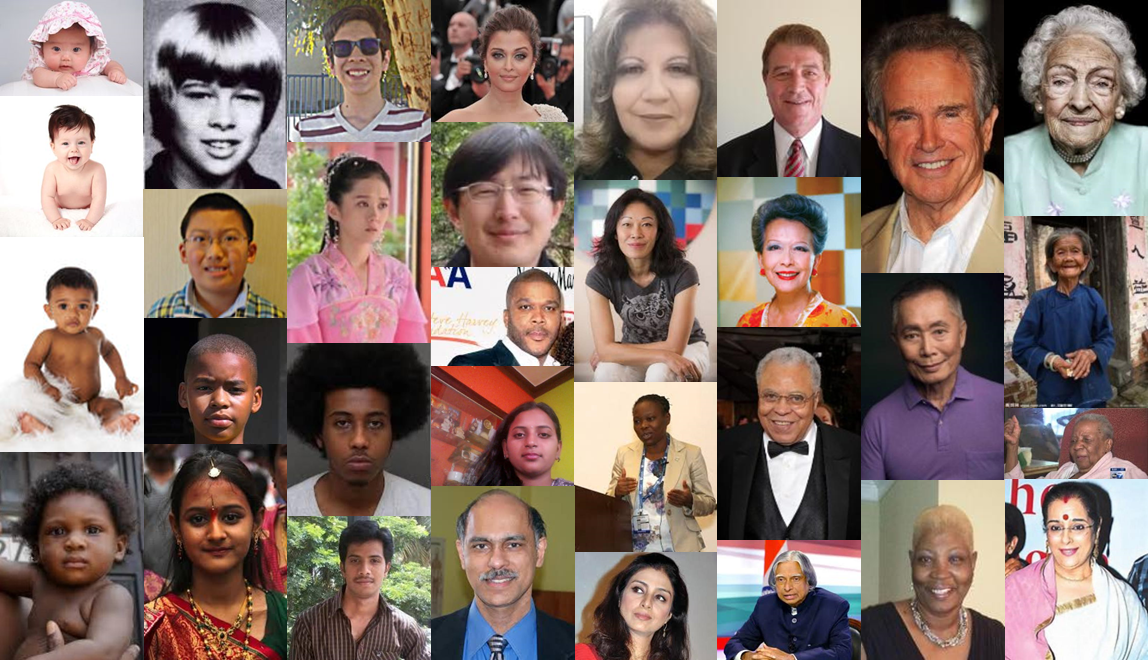
\includegraphics[scale=.3]{figs/exemplos-utk.png}
    \legend{Fonte: \textit{UTKFace dataset} \cite{utkface})}
    \label{fig:exemplos-utk}
 \end{figure}

No primeiro teste, foram filtradas apenas imagens de pessoas entre 18 e 60 anos de idade e executado um teste de detecção de faces sob um grupo aleatório de 5 mil imagens desse grupo, os resultados podem ser vistos na tabela \ref{resultados-teste-1}.

\begin{table}[htbp]
    \caption{Resultados Teste 1.}
    \label{resultados-teste-1}
    \begin{center}
    \begin{tabular}{rrr}\hline\hline
        \text{Número de faces} & \text{Número de imagens} & \text{Porcentagem} \\
        0 & 192 & 5.4763\% \\
        1 & 2659 & 75.8414\% \\
        Mais de 1 & 655 & 18.6823\% \\
    \hline\hline
    \end{tabular}
    \end{center}
\end{table}

No segundo teste, foram novamente filtradas apenas imagens de pessoas entre 18 e 60 anos de idade e desta vez executado um teste de detecção de faces sob todo o grupo que se enquadrava no filtro, sendo um total de 17130 imagens, os resultados podem ser vistos na tabela \ref{resultados-teste-2}.

\begin{table}[htbp]
    \caption{Resultados Teste 2.}
    \label{resultados-teste-2}
    \begin{center}
    \begin{tabular}{rrr}\hline\hline
        \text{Número de faces} & \text{Número de imagens} & \text{Porcentagem} \\
        0 & 891 & 5.2014\% \\
        1 & 13111 & 76.5382\% \\
        Mais de 3128 & 655 & 18.2604\% \\
    \hline\hline
    \end{tabular}
    \end{center}
\end{table}

No terceiro teste, foi novamente executado um teste de detecção de faces sob o mesmo grupo do segundo teste (17130 imagens), mas foram alterados alguns parâmetros do modelo de detecção para que este se tornasse mais sensível, ou seja, detectaria uma maior quantidade de faces, mas com mais chance de ocorrência de falsos positivos, os resultados podem ser vistos na tabela \ref{resultados-teste-3}.

\begin{table}[htbp]
    \caption{Resultados Teste 3.}
    \label{resultados-teste-3}
    \begin{center}
    \begin{tabular}{rrr}\hline\hline
        \text{Número de faces} & \text{Número de imagens} & \text{Porcentagem} \\
        0 & 263 & 1.5353\% \\
        1 & 8439 & 49.2645\% \\
        Mais de 1 & 8428 & 49.2002\% \\
    \hline\hline
    \end{tabular}
    \end{center}
\end{table}
